%% Sample chapter file, for use in a thesis.
%% Don't forget to put the \chapter{...} header onto each file.

\chapter{Background}

	\section{User Centred Design}

		\subsection{Introduction to User Centred Design}

The term User Centred Design was coined and popularized by Donald Norman's research group in the 1980s. Two influential books were published in that time which he co-authored: "User centered system design" \citep{norman1986user} and "The psychology of everyday things" \citep{norman1988design}. UCD is sometimes referred to as User Centred System Design (UCSD). This ambiguity comes from the definition of UCD not being agreed upon for many years \citep{Gulliksen2003}.

User Centred Design (UCD) is a broad term that describes both a philosophy and a set of tools used during the design process \citep{norman1986user, norman2013design}. At its core, it gives central role to the needs and limitations of the user. The level of involvement of the user in the design process may vary, but the fundamental difference compared to other approaches is that decisions are driven by a very deep understanding of users' needs (or even by users themselves). It is not limited to interface optimisation and often means working closely with users already at definition stage where they help in the problem identification. Fundamentally, UCD tries to "focus on usability throughout the entire development process and further throughout the system life cycle" \citep{Gulliksen2003}.

The need for "people oriented" interfaces was already recognized in the early days of computers \citep{ritter2014foundations, nickerson1969man}. Voices of concern were raised that product development methods used at the time were more suitable for big, labour intensive projects and were failing with sophisticated devices which focus on usability \citep{greenbaum1993design, robert1965new}. In 1960s and 1970s there were a number of fields in academia concerned with designing more human friendly devices and processes, but they were applied with varied success. What made UCD so effective was that it "focused on the needs of the user, on activity/task analysis as well as a general requirements analysis, carrying out early testing and evaluation, and designing iteratively." \citep{ritter2014foundations}. It also emphasized the involvement of the user in the design process instead of treating him purely as a consumer of the product. This has been a paradigm shift that was particularly uncomfortable for managers in the United States who were reluctant to hand over the decision making power \citep{greenbaum1993design}.

UCD has changed over the years.  Initially UCD was focused on command-line tools, but as computers got more widespread and their interfaces became more sophisticated, it started growing in importance and played a different role. With Graphical User Interfaces (GUI) it was focused on layouts and optimisation and with nowadays proliferation of computational systems, UCD design is considering things like personal preferences or social and cultural impact of the device \citep{ritter2014foundations}.

		\subsection{Human Centred Design}

Human Centred Design (HCD) is a broader term that puts humans at the centre \citep{ritter2014foundations, Earthy2001, iso199913407, 1_kurosu_2011}. This means taking into consideration the entire context of the situation in which the product will be used and the human aspects of it. It is considered more interdisciplinary than UCD and is described in many standards \citep{Bevan2001} such as ISO 13407:1999 \citep{iso199913407} and more recently 9241-210: 2010 \citep{dis20099241}. UCD is considered by some as being too much focused on solving a goal-directed, technological problem and limited by considering people solely as users of the system without looking at the organisational goal or counteracting possible adverse effects of use on human health, safety and performance \citep{gasson2003human, gill1996foundations, Bevan2001}. UCD and HCD are not synonyms and HCD does not necessarily imply using UCD methods \citep{Earthy2001, Maguire2001, 1_kurosu_2011, ritter2014foundations}. 
		
		\subsection{Design Driven Innovation}

A recent perspective that is broadening the definition of design to include a reconstructionist \citep{chan2005blue} or social-constructionist \citep{Prahalad2000} view of the market is Design Driven Innovation \citep{Liem2011, verganti2013design}.   

In his book "Design driven innovation: changing the rules of competition by radically innovating what things mean" Roberto Verganti introduces the concept of Design Driven Innovation \citep{verganti2013design}. In his opinion, most organisations understand and use design in two ways: making things beautiful and stylish and having a profound (and thus accurate) understanding of user needs. Innovations coming from these two, beauty of the product and user needs (which is an embodiment of User Centred Design), are in his opinion insufficient for market differentiation and have become so common that they are a norm rather than exception. Verganti argues that what is needed (together with the first two) is a third use for design which is a radical innovation in meaning.

His research reveals that recent management literature focuses on technological innovation and what effect it has on an industry. What is also very well covered is looking beyond features and understanding the meanings behind them - what emotions drive people to buy products. However, the silent assumption is, he continues, that meanings are not a subject of innovation. He proposes a third strategy for design which is innovation in what meaning things can carry.

The author brings and analyses dozens of examples to help better understand design-driven innovation such as:

\begin{itemize}
\item Artemide, Italian lamp manufacturer, created a lamp that is no longer a source of light, but an object that has influence on people's mood. Effectively, by providing a device that can change intensity and colour of the light you are enabling people to control their mood and the product becomes an element of well-being.

\item The MP3 players were present before iTunes, but it was a change in how to think about music brought by Steve Jobs that revolutionised the industry. Many executives and lobbing groups stubbornly focused on enforcing copy-protection, whereas Apple enabled users to buy a single song instead of an entire album, taste and mix music, create personal playlists.

\item Anthropomorphism in the shape of kitchen appliances brought by Alessi, turned equipment into objects of affection, things you bond with, "teddy bears for adults" \citep{verganti2013design}.

\item Apple's move to release a notebook without an optical drive was considered a bold one, but Steve Job had an understanding of what cloud computing and wireless connectivity meant – constant access to vast amounts of data and thus no use for CDs/DVDs.
\end{itemize}

The author also provides a structured framework for thinking about innovation in meaning and deploying it in an organisation. Design Driven Innovation extends beyond User Centred Design, but does not discredit it.

	\section{Data-driven design}
	
Data-driven design is an emerging field of study that gained popularity with the digitization of our world and in particular with what is known as big data. The premise of data-driven design is an additional layer of perception provided by data collection and processing, previously unavailable to humans. Although the practices of data-driven design are far from being well established, more and more voices are being raised that consider it a very viable tool when used properly with other methods \citep{Neirotti2014}.
	
		\subsection{What would a cup say if it could speak?}

Data can be used to drive the design of many things. Common areas of use of data-driven design in Informatics include websites (web analytics) or mobile apps. A designer can change the layout of a website and in real time analyse what impact on the behaviour of the user it has \citep{CSIRO2015}.

However, computational systems are being used for much more than just reading websites. Vizie is a tool analysing social media feeds and it is able to inform government institutions about a failure of a service, provide situational awareness in emergencies or simply help being in touch with citizens by informing about major topics of the day \citep{CSIRO2015a}. In one case, social media is actually the main, preferred way of communicating with a government institution – for better or for worse \citep{MITMediaLab2015}.

The Internet of Things (IoT) is another case of digitization entering our lives. We are instrumenting objects in our surroundings "giving them a voice". IoT devices will generate a lot of data about their users and the devices themselves. Vessyl is an IoT cup designed to be part of a bigger health and wellness ecosystem. It traces the nutritional value of liquids consumed by the user \citep{MarkOne2014}. Interesting questions arise from the designers' perspective with the emergence of such devices. What impact on the design of the cup do the consumption habits of its users have? If the cup could capture detailed data about its usage patterns – location, acceleration, angle of tilt – could it suggest a better design (e.g. thinner, taller, rounded edges)? Maybe the cup would tell us something else, unrelated to the drink, something that we cannot think of simply because we are humans?

This vast amount of data captured in different areas of people's lives provides a lot of opportunities for generating design insights. It is important to stress that having data by itself is not sufficient. It is what follows – data analysis – that makes all the difference and that is where uncharted territories are.

			\subsubsection{What is big data?}

There are many definitions of what Big Data is and in some cases not only do they differ, but even stand in contradiction. This might be due to the fact that early cases of use of the term happened in different fields \citep{demchenko2014defining, Ward2013}. Most commonly, Big Data is associated with data storage and data analysis, which in themselves are not new concepts at all. A description that is widely accepted as fundamental in coining the term Big Data is the "3 Vs" definition provided by Gartner in 2001 \citep{douglas20013d, Ward2013}. Since then, the "Vs" description has been used and expanded (to "5 Vs") by many \citep{McAfee2012, minelli2012big, demchenko2014defining, NIST2015}.

The "5Vs" of big data are as follows:
\begin{itemize}
\item Volume – 90\% of world's data was generated over the last two years; by some, big data is considered when dealing with volumes over peta bytes ($10^{15}$)

\item Velocity – more data being received than can be processed using "traditional" data analysis approach; you receive more information than you can process before a decision has to be made; processing of real-time data streams is becoming essential

\item Variety – different types of data are being accessible (structured data, sensory data, social media data, voice recordings, photos, videos)

\item Veracity (validity) – lack of control over quality and accuracy which leads to inconsistencies and incompleteness

\item Value – how to get value out of data
\end{itemize}

		\subsection{Data Analysis}
		
Data analysis is a process of cleaning and inspecting data using tools such as modeling, reasoning, processing and visualising. It is a complex activity that can be done with different objectives in mind, e.g. discovering relations, supporting decision making by delivering business insights, designing systems and processes, delivering services and products.

Due to the amount of data that is usually processed when doing data analysis as well as complexity of this task Artificial Intelligence (AI) algorithms are deployed. Fields of AI that are most often used for data analysis include Machine Learning (ML) and Pattern Recognition (PR) \citep{bishop2006pattern}. They have many uses with structured and unstructured data. Some of those relevant in this context include: text/speech recognition, customer choices analysis, usage patterns analysis, decision support systems involving judgment, load forecasting, marketing and sales \citep{witten2005data}.
			
			\subsubsection{Business Intelligence}
Another Data Analysis technique, which is focused on delivering business insights is Business Intelligence (BI). The term was coined by Howard Dresner from Gartner Group in 1989. It describes a set of data-driven tools and practices that emerged from Decision Support Systems (DSS) which went through a time of intense development in 1980's \citep{power2008decision}. BI has been a very popular and dynamic field in recent years which is attributed to, among many others, "more turbulent business environments" and higher demands for profitability \citep{sacu2010bidm, power2008decision, baars2008management}. A range of BI tools that are becoming popular recently are the user-driven solutions which promote "self-service" as opposed to dependence on IT department's involvement \citep{IBM2015a, Qlik2015, Microsoft2015, imhoff2011self}.

The goal of BI is to unveil valid risks and performance indicators, through the means of interpretation (processing) of large volumes of data, in order to support managers on all levels: strategic, tactical and operational \citep{baars2008management}.

There are numerous models describing BI maturity. In general, they take into consideration the following concepts: deployment, use and impact of BI in an organisation \citep{Lahrmann2011}.

Currently most widely used tools within BI are reporting, data mining and Online Analytical Processing (OLAP). In many areas this is insufficient as a lot of data is not numerical or otherwise referred to as unstructured, e.g. voice transcripts, comments, e-mails, documents. This is especially true for analysing data about interactions with customers such as data from Customer Relationship Management (CRM) systems \citep{baars2008management}. There are different approaches and frameworks for building systems that incorporate both data types. In general, they can either process unstructured data to extract from it information in a more structured way (e.g. text processing), present both data types next to each other without processing unstructured data (e.g. show all e-mails relevant to a performance indicator to allow human to understand the situation) or anything in between.

		\subsection{Smart Cities}
Data is considered to be an essential asset in Smart Cities (SC). They make use of it and in many initiatives it plays a major role in the design and operations of city services.

SC try to improve the lives of citizens by creating more sustainable and more efficient urban environment for people to live in \citep{geertman2015planning}. Using technology-based solutions they try to address some of the challenges faced by metropolitan areas \citep{Neirotti2014}. Although there is no clear definition yet of what a SC is, it is widely accepted that Information and Communications Technologies (ICT) play a major role in SC by acting as their "nervous system" \citep{Neirotti2014, geertman2015planning}. Data about different aspects of functioning of the city will be collected, analysed and acted upon in real time. However, ICT capabilities by themselves are not sufficient and have to be matched with adequate human and organisational capital in order to enable cities to act accordingly.  Some research suggest that globally, initiatives within SC are highly diverse and depend heavily on the cultural and socio-economic background of the geographical region making it non trivial to find commonalities, but with time a few archetype models will emerge \citep{Neirotti2014, geertman2015planning}. The highest number of initiatives in area of SC has been observed in "Natural resources and energy" and "Transport and mobility" \citep{Neirotti2014}.

Transportation in Nairobi, Kenya using semi-formal mini-buses has been a subject of a project that used GPS data to improve route planning and way finding \citep{klopp2015leveraging}. The location data was not acquired through telecommunications operators, but was willingly shared by users via a smartphone app. It was made public in GTFS format and processed using open-source tools such as Open Trip Planner \citep{klopp2015leveraging}. It is an example of "bottom-up" approach in which citizens are empowered (Open Data) and supported by local authorities to act and improve their city \citep{Neirotti2014}.

In 2012 the New York City Council has approved a law requiring all city agencies to open their data by 2018. One of the agencies helping in this process is Mayor's Office of Data Analytics (MODA). MODA is responsible for initiatives within five categories: Supporting Operations, Citywide Data Sharing, Disaster Response and Resiliency, Economic Development, Open Data. They are offering courses to other City government employees about data and tools available to them and are also promoting data driven decision making \citep{NYCMODA2014}. One interesting project in New York City is called "Hudson Yards Redevelopment Project" in which an entire part of the city will be built from scratch. It will be collecting information about air quality, pedestrian traffic, energy production and consumption. It will have a trash-disposal system to remove waste via underground pneumatic tubes.

	\section{Double Diamond}
	
"Double Diamond" is a model of the design process developed by the UK Design Council \citep{council2007eleven, council2005double}. It is a result of a qualitative study of practices in companies focused on innovation and it describes the commonalities in the creative activities that can be observed among designers regardless of the field they are working in. The model divides the design process into four phases as pictured in Figure 2.1. Each of those phases is focused on a different objective and involves methods which are characteristic to that stage.

\begin{center}
  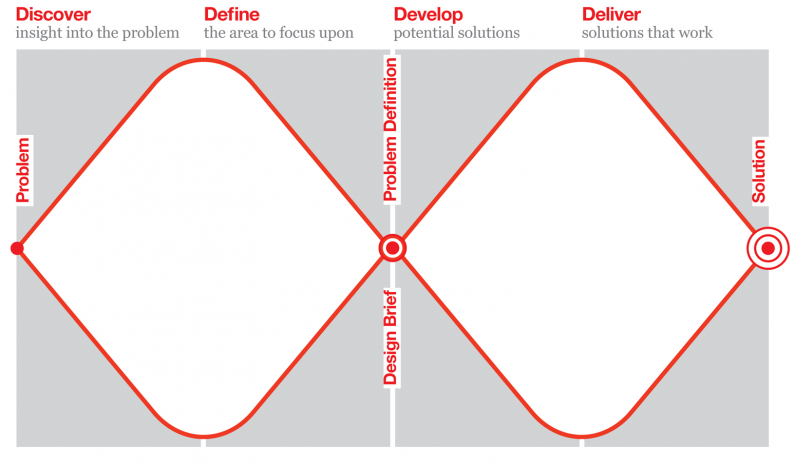
\includegraphics[width=1.0\textwidth]{Double-Diamond-A3-for-publication-A-2000px_1.png}
  \captionof{figure}{Double Diamond model \citep{council2005double} }
\end{center}

		\subsection{Discover}

At this stage the attitude adopted is of openness in terms of thoughts and ideas. All ideas are welcome, different perspectives are nurtured and every direction has the potential to be valid. This thinking is typical at the beginning of the project. Designers try to remain as open as possible so that their own perspectives do not limit creativity. This helps in noticing things that might matter, clues about what would make the situation better especially that it might be something unexpected or not identified.

Some of the activities used at this stage include:
\begin{itemize}
\item Observation
\item User diaries
\item Being your users
\item Brainstorming
\item Choosing a sample
\item Quantitative surveys
\item Fast visualisation
\item Secondary research
\item Hopes and fears
\item Market research
\item User research
\item Managing information
\item Design research groups
\end{itemize}

		\subsection{Define}
		
Second phase is trying to make sense out of all the information collected. It is focused on identifying causalities, narrowing down insights and establishing the main challenge which will be addressed. It takes into consideration limitations of the project in terms of what is feasible given the time and resources. Selection and discarding of ideas takes place here as well. It starts with numerous concepts and ideas and finishes with a clear definition of the problem and a list of actionable tasks.

Activities at this stage often involve:
\begin{itemize}
\item Focus groups
\item Assessment criteria
\item Comparing notes
\item Drivers and hurdles
\item Customer journey mapping
\item Project development
\item Project management
\item Project sign-off
\end{itemize}

		
		\subsection{Develop}
		
This stage involves intense creation, prototyping and testing. It takes the results of the previous phase as a "design brief" and uses it as a framework for the development process. Iterating is very important in order to improve and refine the prototypes as well as concepts. Attitude of trying and failing ensures the space for testing different implementations using different techniques and thus finding the best one. Some of the tools used are similar to Define stage, but here they are focused on bringing a product ready for production.

Typical to this stage are:
\begin{itemize}
\item Character profiles
\item Scenarios
\item Role-playing
\item Service blueprints
\item Physical prototyping
\item Multi-disciplinary working
\item Visual management
\item Development methods
\item Testing
\end{itemize}		
		
		\subsection{Deliver}

The last phase is when the product is being finalised, produced and launched. Here it is mass produced, checked before release and delivered to the user. Feedback mechanisms should be in place which will improve the product itself, but also methods and practices used in the process of creation of it.

Characteristic to this phase are the following activities:
\begin{itemize}
\item Phasing
\item Final testing
\item Evaluation
\item Feedback loops
\item Methods banks
\item Approval
\item Launch
\item Targets
\end{itemize}



